

\section{Review of State-wise Safe Reinforcement Learning}

The existing research on state-wise safe RL can be divided into two categories based on whether safety is ensured during training.
\begin{itemize}
    \item \textbf{State-wise safety after convergence.} When a policy converges, it ensures state-wise safety. But the policy may be unsafe during training.
    \item \textbf{State-wise safety during training.} The policy derived from this class of methods always ensures constraint satisfaction, even during training.
\end{itemize}
In addition, each category can be further classified into two approaches: hierarchical agents and end-to-end agents.
In the following sections, we will explore these categories through the lens of these two approaches.

\subsection{State-wise Safety After Convergence}

\begin{figure}[htbp]
    \centering
    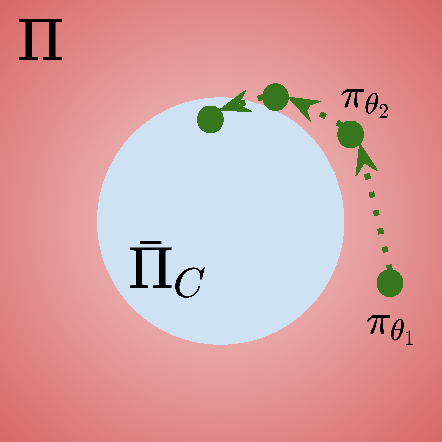
\includegraphics[width=0.2\textwidth]{figs/p1.pdf}
    \caption{State-wise safety after convergence}
    \label{fig:state-wise-safety-after-convergence}
\end{figure}
State-wise safety after convergence refers to methods that have possibl infeasible policies during training and feasible converged stationary policies in the end.
As shown in \autoref{fig:state-wise-safety-after-convergence}, this class of methods uses soft penalties (typically called safe critic $Q_C(s, a)$) to guide the training of policies.
The safety critic $Q_C(s, a)$ can be provided by humans or learned from the envrionment.
This class of methods does not pose hard constraints on the exploration space, therefore the policy learning can be made efficient.
Nevertheless, the policy may be unsafe during training and the convergence to $\Pi_C$.

\subsubsection{Hierarchical Agent}

\subsubsection{End-to-End Agent}

\subsection{State-wise Safety During Training}


\begin{figure}[htbp]
    \centering
    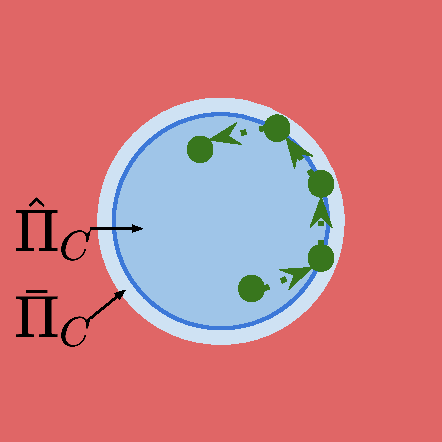
\includegraphics[width=0.2\textwidth]{figs/p2.pdf}
    \caption{State-wise safety during training by constraining policies in a subset of $\bar{\Pi}_C$}
    \label{fig:state-wise-safety-during-training-constraint}
\end{figure}
We denote the policy sequence during training as $\pi_{\theta_1}, \pi_{\theta_2}, \cdots, \pi_{\theta_n}$, where $\theta_i$ represents the policy parameters at the i-th optimization iteration, and n is the total number of iterations.
State-wise safety during training requires that all intermediate policies satisfy the constraint, i.e., $\pi_{\theta_i} \in \bar{\Pi}_C$ for all $i \leq n$.
Becuause it requires all intermediate policies during training to be feasible.

As shown in \autoref{fig:state-wise-safety-during-training-constraint}, the first class defines a subset of $\bar{\Pi}_C : \hat{\Pi}_C$ (typically by control barrier functions).
Whenever the policy goes out of the subset, it will be projected back.
Therefore the policy is always guaranteed to be safe during training.
However, $\hat{\Pi}_C$ requires a significant amount of prior knowledge about the environment, which may be lacking in many cases.
And in general, these methods are conservative than after-convergence methods.

\begin{figure}[htbp]
    \centering
    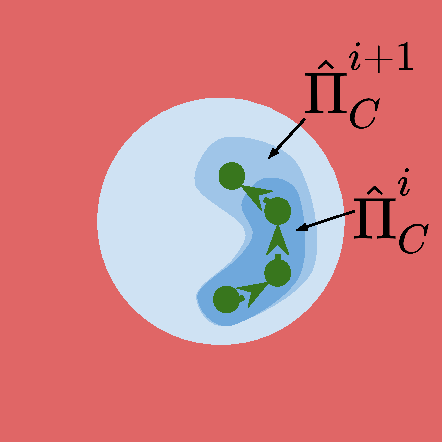
\includegraphics[width=0.2\textwidth]{figs/p3.pdf}
    \caption{State-wise safety during training by progressive safe exploration}
    \label{fig:state-wise-safety-during-training-progressive}
\end{figure}
Second class of methods progressively explores the policy space from a safe initial policy as shown in \autoref{fig:state-wise-safety-during-training-progressive}.
This class of methods maintains an up-to-date subset of $\bar{\Pi}_C : \hat{\Pi}_C$ by exploring and gathering information.
The policy updates in $\hat{\Pi}^{i + 1}_C$ only if there is enough information to confirm that the $\hat{\Pi}^{i + 1}_C \subseteq \bar{\Pi}_C$.
This class of methods requires less prior knowledge than the first class but is more conservative in exploration.